\graphicspath{{chapters/19/images}}
\chapter{Rare events}

\section{Introduction}

	\subsection{Rough free energy surfaces}

	\begin{figure}[H]
		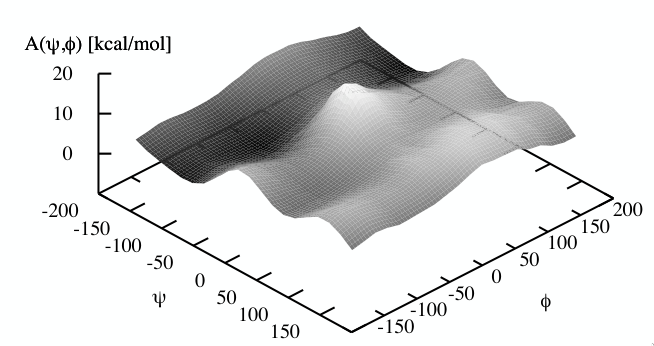
\includegraphics[width=\textwidth]{rough-free-energy-surfaces}
		\caption{Rough free energy surfaces}
		\label{fig:rough-free-energy-surfaces}
	\end{figure}

	\subsection{?????????}

		\begin{itemize}
			\item Reaction coordinates.
			\item Order parameters.
			\item COLVARs.
		\end{itemize}

\section{Reaction coordinates}
Example: $r = |\vec{r}_B-\vec{r}_A|$ for a dissociation reaction $AB\rightarrow A+B$.
Example radius of gyration:

$$R_G = \sqrt{\frac{1}{N_b}\sum\limits_{i=1}^{N_b}\biggl(\vec{r}_i-\frac{1}{N_b}\sum\limits_{j=1}^{N_b}\vec{r}_j\biggr)^2}$$

Example: number of hydrogen bonds of length $d_0$ between $n_O$ oxygens and $n_H$ hydrogens:

$$N_H = \sum\limits_{i=1}^{n_O}\sum\limits_{j=1}^{n_H}\frac{1-\biggl[\frac{\vec{r}_i-\vec{r}_j}{d_0}\biggr]^6}{1-\biggl[\frac{\vec{r}_i-\vec{r}_j}{d_0}\biggr]^{12}}$$

The aim is to obtain the probability distribution function of a subset of $n$ reaction coordinates of interest $q_\alpha= f_\alpha(\vec{r}_1, \dots, \vec{r}_N)$ with $\alpha = 1, \dots, n$:

$$P(s_1, \dots, s_n) = \frac{C_N}{Q(N, V, T)}\int d^N\vec{p}d^B\vec{r}e^{-\beta\mathcal{H}(\vec{r}, \vec{p})}\prod\limits_{\alpha=1}^n\delta(f_\alpha(\vec{r}_1, \dots, \vec{r}_N)-s_\alpha)$$

Free energy hypersurface:

$$A(s_1, \dots, s_n) = -fT\ln P(s_1, \dots, s_n)$$

	\subsection{Blue moon ensemble}
	Single reaction coordinate $q_1 = f_1(\vec{r}_1, \dots, \vec{r}_N)$:

	$$P(s) = \frac{C_N}{Q(N, V, T)}\int d^N\vec{p}d^N\vec{r}e^{-\beta\mathcal{H}(\vec{r}, \vec{p})}\delta(f_1(\vec{r}_1, \dots, \vec{r}_N)-s)$$

	$$A(s) = -kT\ln P(s)$$

	Introduce a holonomic constraint $\sigma(\vec{r}_1, \dots, \vec{r}_N) = f_1(\vec{r}_1, \dots, \vec{r}_N)-s$.
	Use this constraint to drive the reaction coordinate from an initial value $s^{(i)}$ to a final value $s^{(f)}$.
	The blue moon ensemble yields $\frac{dA}{ds} = -\frac{kT}{P(s)}\frac{dP}{ds}$.

	$$A(q) = A(s^{(i)}) + \int_{s^{(i)}}^q\frac{dA}{ds}ds\qquad \Delta A = \int_{s^{(i)}}^{s^{(f)}}\frac{dA}{ds}ds$$

	$$P(s) = \frac{C_N}{Q(N, V, T)}\int d^N\vec{p}d^N\vec{r}e^{-\beta\mathcal{H}(\vec{r}, \vec{p})}\delta(f_1(\vec{r}_1, \dots, \vec{r}_N)-s) = \langle\delta(f_1(\vec{r}_1, \dots, \vec{r}_N)-s)\rangle$$

	$$\frac{1}{P(s)}\frac{dP}{ds} = \frac{C_N}{Q(N, V, T)}\frac{\int d^N\vec{p}d^N\vec{r}e^{-\beta\mathcal{H}(\vec{r}, \vec{p})}\frac{\partial\delta(f_1(\vec{r})-s)}{\partial s}}{\langle\delta(f_1(\vec{r})-s)\rangle}$$

	Introduce $3N$ generalized coordinates $q_\alpha = f_\alpha(\vec{r}_1, \dots, \vec{r}_N)$ and their conjugate momenta $p_\alpha$,
	The transformation is canonical, hence: $d^N\vec{p}d^N\vec{r} = d^{3N}pd^{3N}q$:

	$$\frac{1}{P(s)}\frac{dP}{ds} = \frac{C_N}{Q(N, V, T)}\frac{\int d^{3N}pd^{3N}qe^{-\beta\tilde{\mathcal{H}}(q, p)}\frac{\partial\delta(q_1-s)}{\partial s}}{\langle\delta(q-s)\rangle}$$

	However $\frac{\partial}{\partial s}\delta(q_1-s) = -\frac{\partial}{\partial q_1}\delta(q_1-s)$.
	Integrating by parts:

	\begin{align*}
		\frac{1}{P(s)}\frac{dP}{ds} &=-\frac{\beta C_N}{Q(N, V, T)}\frac{\int d^{3N}pd^{3n}q\frac{\partial\tilde{\mathcal{H}}}{\partial q_1}e^{-\beta\tilde{\mathcal{H}}(q, p)}\delta(q_1-s)}{\langle\delta(q_1-s)\rangle} = \\
																&= -\frac{\beta}{\langle\delta(q_1-s)\rangle}\biggl\langle\frac{\partial\tilde{\mathcal{H}}}{\partial q_1}\delta(q_1-s)\biggr\rangle \equiv -\beta\biggl\langle\frac{\partial\tilde{\mathcal{H}}}{\partial q_1}\biggr\rangle^{cond}
	\end{align*}

	$$A(q) = A(s^{(i)}) + \int_{s^{(i)}}^q\biggl\langle\frac{\partial\tilde{\mathcal{H}}}{\partial q_1}\biggr\rangle^{cond}_sds$$


	\subsection{Umbrella sampling}

	\subsection{WHAM}

	\subsection{Wang-Landau sampling}
